\documentclass{article}
\usepackage[utf8]{inputenc}
\usepackage{tikz}
\usetikzlibrary{positioning}

\title{Pythagorean Theorem}
\author{1505071}
\date

\begin{document}

\maketitle

\section{Introduction}
In this document, we present the very famous theorem in mathematics: \textit{Pythagorean 
theorem}, which is stated as follows.
\\
\textbf{Theorem 1.1 (Pythagorean theorem)}\textit{The square of the hypotenuse (the
side opposite the right angle) is equal to the sum of the squares of the other two
sides.}
\\
Numerous  mathematicians  proposed  various  proofs  to  the  theorem.   
The theorem was long known even before the time of Pythagoras.  Pythagoras was
the first to provide with a sound proof.  The proof that Pythagoras gave was
by \textit{rearrangement}
.   Even  the  great  Albert  Einstein  also  proved  the  theorem
without \textit{rearrangement}, rather by using dissection.  Figure 1 shows the visual
representation of the theorem.

\vspace{5mm}

\begin{center} 
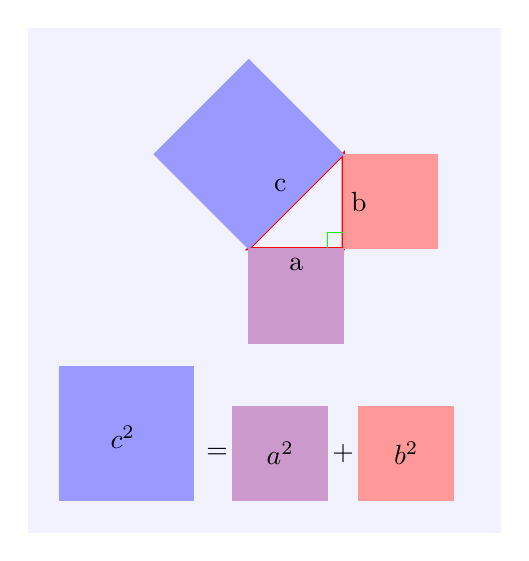
\begin{tikzpicture}[xscale=0.4,yscale=0.4]

\filldraw [color=blue!5](0,0) rectangle (15,16);
\draw[color=red,very thick] (7,9) -- (10,9) -- (10,12) -- cycle;
\draw [green] (9.5,9)--(9.5,9.5)--(10,9.5);
\filldraw[color=red!40,fill=red!40] (10,9) rectangle (13,12);
\filldraw[color=violet!40,fill=violet!40] (7,6) rectangle (10,9);
\filldraw[color=blue!40,fill=blue!40] (4,12) -- (7,9) -- (10,12) -- (7,15) -- cycle;
\node[black] at (8,11) {c};
\node[black] at (10.5,10.5) {b};
\node[black] at (8.5,8.5) {a};
\filldraw[color=blue!40,fill=blue!40] (1,1) rectangle (5.243,5.243);
\filldraw[color=violet!40,fill=violet!40] (6.5,1) rectangle (9.5,4);
\filldraw[color=red!40,fill=red!40] (10.5,1) rectangle (13.5,4);
\node[black] at (3,3) {$c^2$};
\node[black] at (8,2.5) {$a^2$};
\node[black] at (12,2.5) {$b^2$};
\node[black] at (6,2.5) {$=$};
\node[black] at (10,2.5) {$+$};
\end{tikzpicture}
\end{center} 

\begin{center}
Figure 1: Visual representation of the famous Pythagorean theorem.
\end{center}

\newpage

\begin{center} 
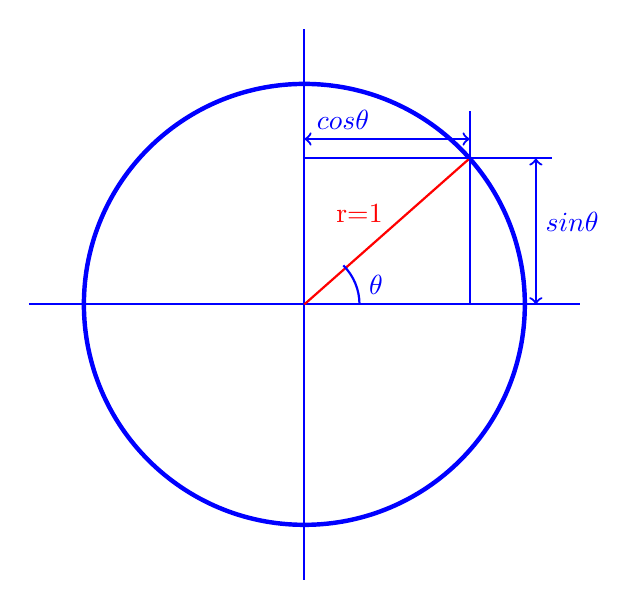
\begin{tikzpicture}[xscale=0.7,yscale=0.7]
%\draw[] (0,0) grid (11,10);
\draw[blue,ultra thick] (5,5) circle(4);
\draw[blue,thick] (0,5) -- (10,5);
\draw[blue,thick] (5,0) -- (5,10);
\draw[red,thick] (5,5) -- (8,7.65);
\draw[blue,thick] (8,5) -- (8,8.5);
\draw[blue,thick] (5,7.65) -- (9.5,7.65);
\draw[blue ,thick,<->] (9.2,5) -- (9.2,7.65);
\draw[blue,thick,<->] (5,8) -- (8,8);
\draw [blue,thick] (6,5) arc [radius=1, start angle=0, end angle= 45];
\node [blue,right] at (9.2,6.5) {$sin\theta$};
\node [blue,above] at (5.7,8) {$cos\theta$};
\node [red,above] at (6,6.3) {r=1};
\node [blue,above] at (6.3,5) {$\theta$};
\end{tikzpicture}
\end{center} 

\begin{center}
Figure 2: Alternate representation of Pythagorean theorem.
\end{center}

\section{Trigonometric Forms}
Lots of other forms of the same theorem exist.  The most useful, perhaps, are
expressed in trigonometric terms, as follows:

\begin{equation} \label{eq1}
sin^2\theta+cos^2\theta=1
\end{equation}

\begin{equation} \label{eq2}
sec^2\theta-tan^2\theta=1
\end{equation}

\begin{equation} \label{eq3}
cosec^2\theta-cot^2\theta=1
\end{equation}

\subsection{Representing the First}
Taking 1,  we can show them as shown in Figure2.  When we take a point at
unit distance from the origin, the y and x co-ordinates become $sin\theta$ and $cos\theta$
respectively.   Therefore,  sum  of  the  squares  of  the  two  becomes  equal  to  the
square of the unit distance, which of course, is 1.

\end{document}

